% http://www.idsc.ethz.ch/education/theses-semester-projects.html
% IDSC LaTeX Thesis Template
% 
% Author(s):	Eric Müller
% 				Institute for Dynamic Systems and Control
% 				Swiss Federal Institute of Technology (ETH) Zurich
% 
% Created:		2004/04/02  (Eric Mueller)
% 
% Notes: Has been tested on Windows 7 + MikTeX + TeXnicCenter
%
% Revisions: 	2009/05/29  (Soren Ebbesen)
% 				    2011/03/22	(Soren Ebbesen)
%             2013/03/08	(Soren Ebbesen)
%             2014/03/13	(Soren Ebbesen)
% ______________________________________________________________________________
\documentclass[12pt,twoside,a4paper]{report}
\usepackage{siunitx}
\usepackage[onehalfspacing]{setspace}
%\usepackage{lineno}\linenumbers
\usepackage{pdfpages}
\usepackage{algorithm}
\usepackage{algpseudocode}
\usepackage{amsmath,mathtools}

% CHANGE HERE FOR GERMAN (german) OR MASTER THESIS (mt)!!!!!
\usepackage[english,mt]{ethidsc} % Special IDSC styles and commands      	
								 % {german}/english: language of headings, etc.
								 % {st}/bt/mt: {semester}/bachelor/master thesis

% Page header (don't change)____________________________________________________
\setlength{\parindent}{0em}                 % Disable parindent
\rhead[\nouppercase{\rightmark}]{\thepage}  % Special headings
\lhead[\thepage]{\nouppercase{\leftmark}}   % Special headings
\cfoot{}                                    % Special headings


% ---------------------------------------------------------------------------------------------------------------
% ---------------------------------------------------------------------------------------------------------------

% https://tex.stackexchange.com/questions/67908/customizing-the-algorithmic-package-break-and-loop-labels
\makeatletter
\newcommand{\ALOOP}[1]{\ALC@it\algorithmicloop\ #1%
  \begin{ALC@loop}}
\newcommand{\ENDALOOP}{\end{ALC@loop}\ALC@it\algorithmicendloop}
\renewcommand{\algorithmicrequire}{\textbf{Input:}}
\renewcommand{\algorithmicensure}{\textbf{Output:}}
\newcommand{\algorithmicbreak}{\textbf{break}}
\newcommand{\BREAK}{\STATE \algorithmicbreak}
\makeatother

% https://tex.stackexchange.com/questions/208119/how-to-make-whiletrue-do-loop
\newcommand{\sfunction}[1]{\textsf{\textsc{#1}}}
\algrenewcommand\algorithmicforall{\textbf{foreach}}
\algrenewcommand\algorithmicindent{.8em}


% ---------------------------------------------------------------------------------------------------------------
% ---------------------------------------------------------------------------------------------------------------

% Title page (please fill in)___________________________________________________
\title{Simulation of mechanical weathering for modeling rocky terrains}

\studentA{Diego Mateos}
\ethidA{20-000-00}
\semesterA{6}
\emailA{diego.mateos@estudiantat.upc.edu}

\supervision{Prof. Dr. Oscar Argudo Medrano}
% \supervision{Prof. Dr. Antonio Susin Sanchez}
\date{October 12, 2023}

%\identification{IDSC-XX-YY-ZZ} 		% Project identifier


% ---------------------------------------------------------------------------------------------------------------
% Begin document________________________________________________________________
\begin{document}

% appears shifted! added later with an external tool
% 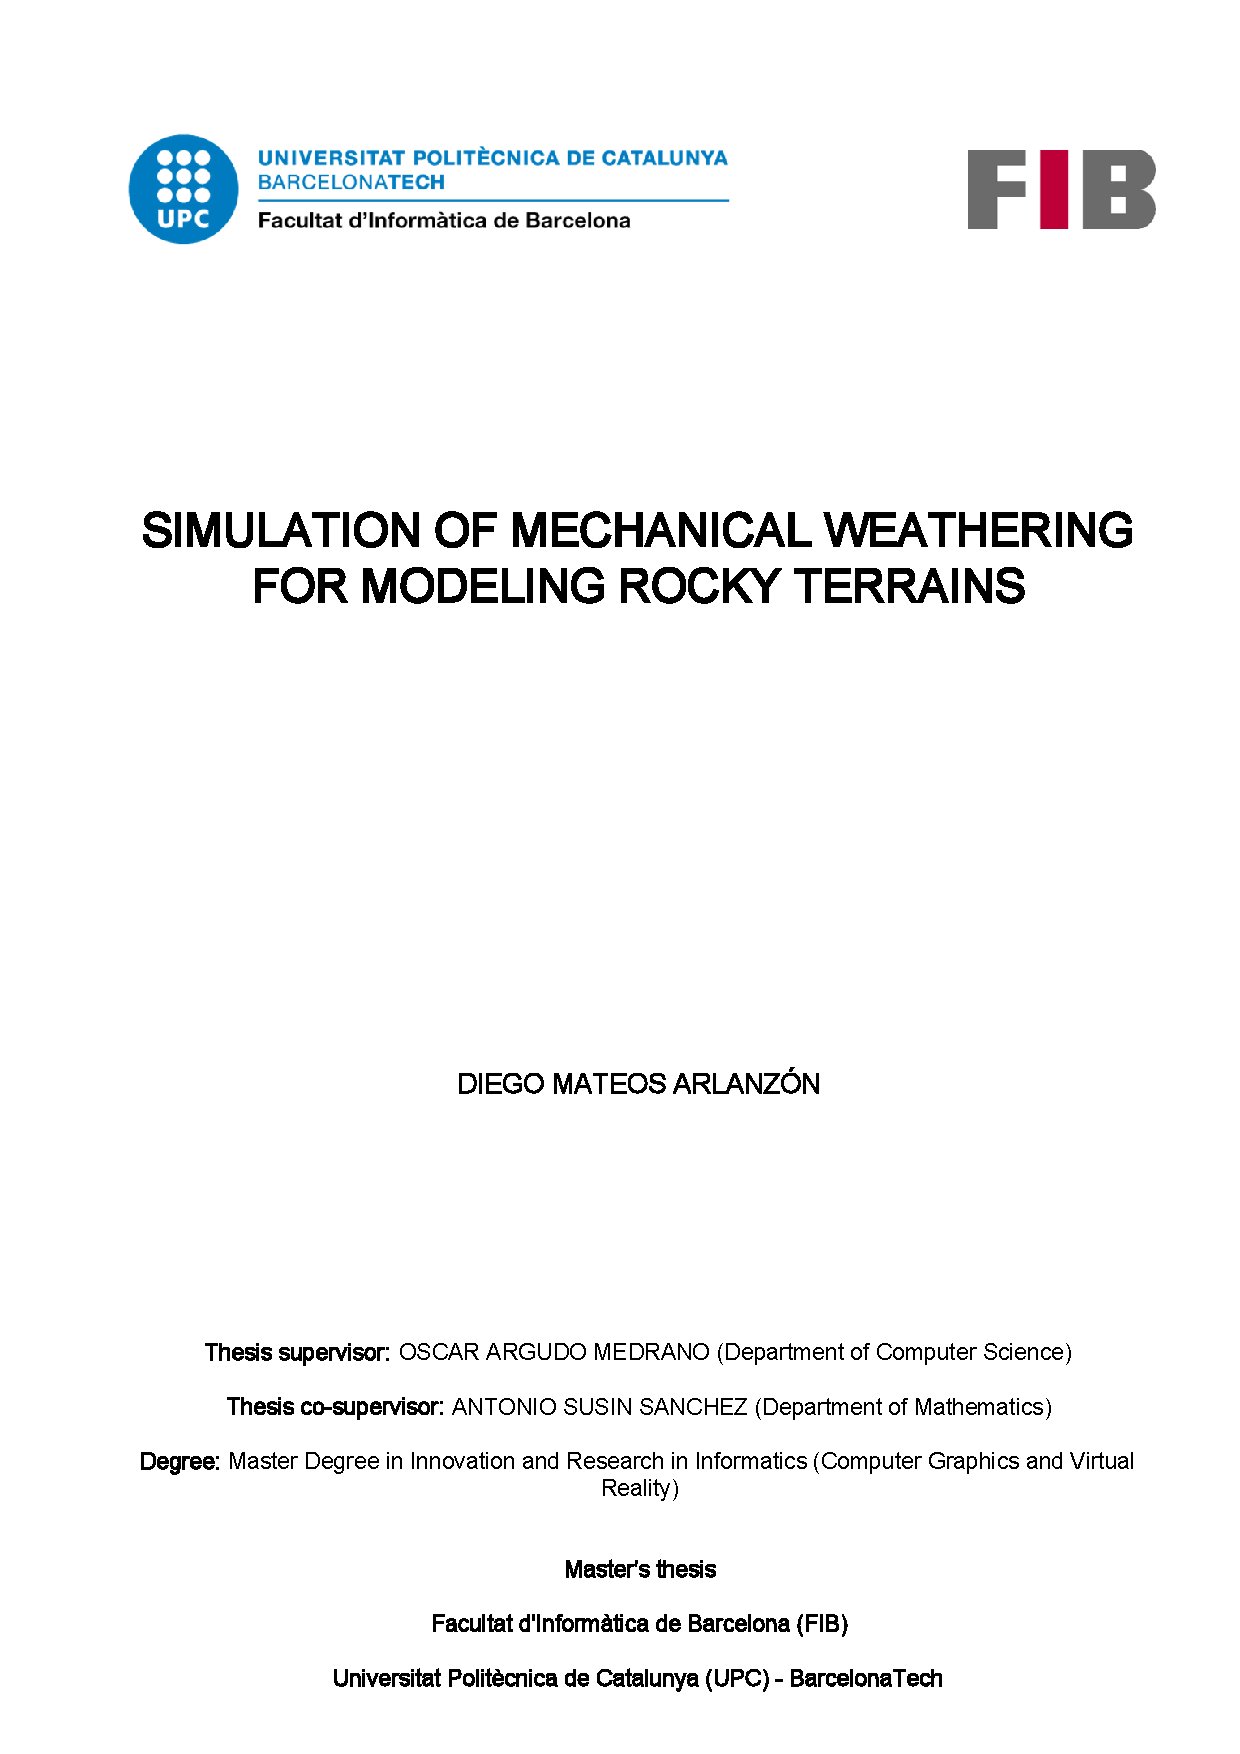
\includepdf[pages={1}]{portada.pdf}

% Preamble______________________________________________________________________
\pagenumbering{roman} 				% Begin roman page numbering (i,ii,...)

%---------------------------------------------------------------------------
% Abstract

\chapter*{Abstract}
 \addcontentsline{toc}{chapter}{Abstract}

Synthetic terrains play a vital role in various applications, including entertainment, training, and simulation. While significant progress has been made in terrain generation, existing methods often focus on large-scale features, relying on 2D elevation maps to model them. However, rocky terrains like those found in alpine environments have many detail features like sharp ridges, loose blocks or overhangs that are poorly represented in this maps, so it is common to model them using textures. 

\vspace{0.5\baselineskip}
Instead, in this project, we aim to generate plausible rocky geometry on top of existing 3D models. We propose a method based on a simplified simulation of mechanical erosion processes commonly found in high altitude terrains such as percolation and freeze-thaw weathering. The process can be controlled through a series of intuitive parameters and its iterative nature lets an artist apply it multiple times until sufficient erosion is achieved.

\vspace{0.5\baselineskip}
Additionally, we developed an artist-friendly tool integrated as add-on into Blender, which is a widely used 3D modeling software. This rich integration streamlines their workflow, eliminating the need for external applications and facilitating direct interaction with the model geometry before and after the simulated erosion.

\vspace{0.5\baselineskip}
\begin{itemize}
    \item \textbf{Keywords}: Computer Graphics, 3D Modelling, Computer Simulation, Rocky Terrains, Mechanical Weathering.
    % \item \textbf{CATALAN}: Gràfics per ordinador, Modelatge 3D, Simulació per ordinador, Terrenys Pedregosos, Erosió Mecànica.
\end{itemize}

 %\cleardoublepage

%---------------------------------------------------------------------------
% Acknowledgements

\chapter*{Acknowledgements}
 \addcontentsline{toc}{chapter}{Acknowledgements}

\texttt{I would like to thank my supervisors, Oscar and Toni, for their continuous support and valuable feedback.}

\vspace{0.5\baselineskip}
\texttt{I am also thankful to all my family and friends for always being there for me, specially Miriam, your personal support is truly invaluable.}

 %\cleardoublepage

%---------------------------------------------------------------------------
% Table of contents

 \setcounter{tocdepth}{4}
 \tableofcontents

 %\cleardoublepage

%---------------------------------------------------------------------------
% Symbols

\chapter*{Acronyms and Abbreviations}\label{chap:symbole}
 \addcontentsline{toc}{chapter}{Acronyms and Abbreviations}


\begin{tabbing}
 \hspace*{3.2cm}  \= \kill

%write abbreviations like this\\
2D\> Two-dimensional\\
3D\> Three-dimensional\\
AABB\> Axis-Aligned Bounding Box\\
API\> Application Programming Interface\\
BFS\> Breadth-first search\\
CGI\> Computer-Generated Imagery\\
CPU\> Central Processing Unit\\
CSG\> Constructive solid geometry\\
DEM\> Digital Elevation Model\\
GPU\> Graphics Processing Unit\\
UI\> User Interface\\
VR\> Virtual Environment\\

\end{tabbing}

%\cleardoublepage

%---------------------------------------------------------------------------



% ---------------------------------------------------------------------------------------------------------------
% Chapters______________________________________________________________________

\pagestyle{fancy}               	% Fancy headings
\pagenumbering{arabic}				% Begin arabic page numbering (1,2,...)
\setlength{\parindent}{20pt}
% \cleardoublepage

\clearpage
\chapter{Introduction}\label{chapter:introduction}

% ---------------------------------------------------------------------------------------------------------------
% ---------------------------------------------------------------------------------------------------------------
\section{Motivation}

Synthetically generated or enhanced terrains are a fundamental part of virtual scenes, which are widely used across industries like entertainment, training or simulation. Researchers have made progress in creating synthetic terrains using three primary methods: fractal modeling, physical erosion simulation, and synthesis from image samples. However these methods have limitations, the main one stems from a focus on the generation of large-scale terrain features like mountains and valleys. To capture these landforms they rely in 2D elevations maps, which is a representation that lacks vertical resolution and therefore cannot represent features like overhangs, arches or caves. Simultaneously, these maps usually cover large portions of terrain with limited precision, consequently producing a poor representation of some detail features commonly found in rocky terrains such as sharp ridges, loose blocks or steep cliffs.

\vspace{0.5\baselineskip}
Representing truly 3D features like those found in the surface of rocky terrains high detail remains a challenge. These complex rocky structures emerge from a variety of physical processes, including weathering from percolation and freeze-thaw cycles. Furthermore, this formations are influenced by the specific material involved, such as limestone, granite or dolomite. Recent physically inspired techniques have been proposed, but most of them are tailored for low altitude fluvial or coastal terrains were erosion tends to be smoother. In contrast, many of the rock formations found in alpine environments present straight cuts and polyhedral shapes.

\vspace{0.5\baselineskip}
Furthermore, most solutions do not offer artists a tool to integrate into their workflows, instead the authoring process is done in an unfamiliar external application. Once a final export is generated, artists may find it challenging to edit the model in alignment with the appropriate generation process. This disconnection between simulation and editing can limit the creative flexibility and efficiency of artists when working with terrain models.

% ---------------------------------------------------------------------------------------------------------------
% ---------------------------------------------------------------------------------------------------------------
\section{Objectives}

The primary objective of this project is to generate plausible rocky geometry on top of existing 3D models, which could come from 2D elevation maps or any already enhanced technique. We base our method specifically in a simplified simulation of mechanical erosion processes common in high altitude terrains such as percolation and freeze-thaw weathering.

\vspace{0.5\baselineskip}
We also seek to develop an intuitive tool to tune the parameters and interact with the simulation inside a popular 3D modelling software, in this case Blender, which is an open source alternative. This environment will let the artists leverage on their past experience with such kind of software, and so speed up the process of learning how to use the integrated interface. On top of that, having a streamlined workflow inside a single application empowers the artist with a cohesive simplified experience, compared to going back and forth between programs and import/export steps.

% ---------------------------------------------------------------------------------------------------------------
% ---------------------------------------------------------------------------------------------------------------
\section{Contribution}

Our research contributes to the field of terrain generation and 3D modeling by addressing some challenges associated with the creation of realistic rocky features. We propose a method to enhance models with a physically inspired erosion simulation. We also produced a user-friendly tool which is totally integrated inside a popular 3D modelling software (Blender). Overall, this tool allows artists to apply the erosion simulation to a model interactively. All of the parameters can be intuitively tuned to tailor the erosion and achieve satisfying results. This eroded models could potentially improve the quality and authenticity of virtual scenes which, as mentioned, are used in diverse applications across different industries. The key contributions of this work are summarized in the following subsections.

% ---------------------------------------------------------------------------------------------------------------
\subsection{Erosion simulation}

Conceptually, our method can be divided into generation and simulation. The former involves computing the geometry of some initial shards of material and their properties. The latter uses all this information to perform an iterative erosion simulation inspired by percolation and freeze-thaw weathering, which changes the shape of the original model by detaching shards over time. The user has a certain degree of control over both processes through a series of parameters, and also decides when to proceed to the erosion simulation and when to end it.

\vspace{0.5\baselineskip}
For the generation process we used Voronoi shaped shards but any convex decomposition would work, a benefit of Voronoi tessellation is the fact that cells have a more natural rocky appearance than, for example, regular tetrahedra. These shards represent chunks of a continuous material kept together through virtual bonds yet to be fractured by the simulation. Based in the freeze-thaw cycle, we simulate how trapped water between the shards pushes their faces in opposite directions causing internal fractures between them. 

\vspace{0.5\baselineskip}
The state of this internal separation is modeled with virtual \textit{links}, which technically model the bonding \textit{connection} between shards instead of the physical gap. This means that the gap between two shards is inversely proportional to the sanity of their bonding \textit{link}. Therefore when a \textit{link} is broken, it means that the separation has reached certain threshold and we consider the shards no longer attached.

\vspace{0.5\baselineskip}
The simulation process works iteratively. Every iteration starts with water percolation entering the model through an external shard, then continues to propagate through its interior running through the spaces between the shards. We call \textit{path} the route the body of water follows throughout an infiltration. We model paths follow a stochastic flow method, in other words, there is a single path at a time with no water flow division. The internal propagation depends only on its current state, which in essence, can be interpreted as a Markov random walk. 

\vspace{0.5\baselineskip}
Inevitably, part of the water is trapped along the path which will produce weathering due to ice expansion as in a freeze-thaw cycle. In our model, we translate this erosion to a reduction in the sanity of the bonding \textit{links} between cells. After a series of simulated water infiltrations, the sanity of certain \textit{links} decrease enough to be considered broken. We continuously analyse the remaining structure of shards and remove totally disconnected groups from the model.

% ---------------------------------------------------------------------------------------------------------------
\subsection{Blender extension}

We developed a tool integrated into Blender in the form of a full fledged add-on. This environment lets the artists leverage on their past experience with such kind of software, and so speeds up the process of learning how to use the integrated interface. This integration streamlines their workflow, eliminating the need for external applications and facilitating direct interaction with the model geometry before and after the simulated erosion.

\vspace{0.5\baselineskip}
The artist interaction is also divided into two parts, first generating a fracture structure out of an object, and then simulating water infiltrations to erode it. The simulation process is iterative, thus the artist is expected to apply it multiple times until a sufficient erosion state is achieved. All parameters can be edited intuitively through UI panels that also provide relevant information of the simulation state.

\vspace{0.5\baselineskip}
Additionally, over the development process we created a range of utilities to aid ourselves and potentially an advanced end-user. We believe these tools could assist greatly in further research of potential future work. 

\clearpage
\input{chapters/2_Background}
\clearpage
\input{chapters/3_Previous}

\clearpage
\input{chapters/4_Method}
\clearpage
\input{chapters/5_Implementation}

\clearpage
\input{chapters/6_Results}
\clearpage
\chapter{Conclusion}\label{chapter:Conclusion}

In conclusion, this project has addressed challenges found in rocky terrain generation and introduced an innovative approach to generate rocky features directly onto 3D models. The method, inspired by mechanical erosion processes like percolation and freeze-thaw weathering, provides an iterative simulation that can add increasing erosion on demand. On top of that, as demonstrated in the results chapter, a wide range of intuitive parameters can be tuned to tailor the simulation behavior. Overall, this solution could potentially improve the quality and authenticity of virtual scenes which, as mentioned, are used in diverse applications across different industries

\vspace{0.5\baselineskip}
Additionally, we developed an artist-friendly tool integrated as add-on into Blender. This rich integration streamlines their workflow, eliminating the need for external applications and facilitating direct interaction with the model geometry before and after the simulated erosion. All parameters can be edited intuitively through UI panels that also provide relevant information of the simulation state. Moreover, we believe the extensive utilities created could assist greatly in further research and development. 

\vspace{0.5\baselineskip}
Finally, we comprehensively analyzed the limitations found in both the method and implementation. This leaves us with a clear view of the potential future work.


% ---------------------------------------------------------------------------------------------------------------
% ---------------------------------------------------------------------------------------------------------------
\clearpage
\section{Future Work}

Future work could address several limitations depicted in \ref{limitations}. We believe that the missing physics integration is the most damming one. It seems to produce overhanging cells with insufficient support that look unrealistic. Future work should explore the inclusion of the mentioned physics-based interactions.

\vspace{0.5\baselineskip}
Additionally, we also believe artists could get a lot more value out of the tool if we could lift some of the limitations currently present on input models. For example, expanding the current implementation to support non-convex shapes would enhance a lot its versatility. We could also explore an automatic multi-scale recursive approach, which should handle appropriately large pieces of terrain without requiring intensive manual interaction from the user.

\vspace{0.5\baselineskip}
Another avenue for future work would be exploring other kinds of user interactions. For example, we could add a brush tool to control better the entry zone of water and thus force erosion in specific parts of the model. On pair with this brush tool, we could have another one to help artists in the distribution of input points non-uniformly. This would allow them to increase the number of cells produced in specific parts of the model, which will produce a more granular detailed erosion there.

\vspace{0.5\baselineskip}
Finally, the technical issues regarding the implementation could be taken as another direction of future work. This would include the Voronoi precision, Blender serialization and overall performance. All would help by improving the experience for the final user.



% ---------------------------------------------------------------------------------------------------------------
% Appendix______________________________________________________________________
\clearpage
\appendix

% deliver as separated pdf
% \input{chapters/appendix}
% \input{chapters/test}

% Bibliography__________________________________________________________________
% Literature (Additional references can be added to the .bib-file manually, or by using, for example, the free application JabRef). Compile in the following order: latex -bibtex -latex -latex
% \bibliographystyle{plain} % numbered
\bibliographystyle{apalike} % name and year

\clearpage
% \begin{footnotesize} % smaller size
\bibliography{references}
% \end{footnotesize}

\end{document}
